\subsubsection{Physarum Polycephalum}
    %Parrafo 1
    El Physarum Polycephalum, tambi\'en conocido como "The Blob", 
        o "La Mancha", es un protista con formas celulares diversas. El Physarum Polycephalum
        es un mixomiceto acelular, esto proviene de la etapa plasmoidal de su ciclo de vida,
        en la cual el plasmodio es un coenocito multinucleado macroscopico de color amarillo 
        brillante, formado en una red de tubos entrelazados. Esta etapa del ciclo de vida es 
        la que se utiliza para el estudio de este organismo.\cite{Dee1960} Podemos ver un ejemplo
        en la siguiente figura \ref{fig:PhysarumPolycephalum01}.
    \begin{figure}[h]  
        \centering
        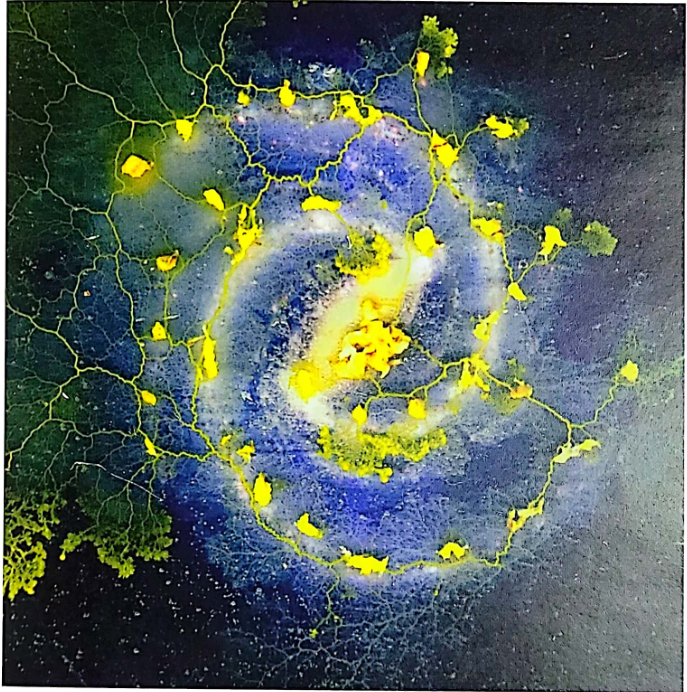
\includegraphics[width=0.5\textwidth]{./images/marco_teorico/Physarum/PhyrasumPolycephalum01.png}
        \caption{Physarum propagandose en una impresion artistica de una galaxia. Imagen extraida de 'Atlas of Physarum Computing' de A. Adamatzky \cite{Adamatzky2014}.}
        \label{fig:PhysarumPolycephalum01}
    \end{figure} 
    \vskip 0.5cm
    %Parrafo 2
    Como vimos con anterioridad los mixomicetos se dividen en dos etapas, el plasmodio y los cuerpos fructiferos.
        El Physarum Polycephalum es un mixomiceto que se encuentra en la etapa plasmodial de su ciclo de vida, 
        en la cual el plasmodio es un coenocito multinucleado macroscopico de color amarillo brillante, formado en una red de tubos entrelazados.
        Esta etapa del ciclo de vida es la que se utiliza para el estudio de este organismo.\cite{Dee1960}
    \begin{wrapfigure}{r}{0.17\textwidth}
        \centering
        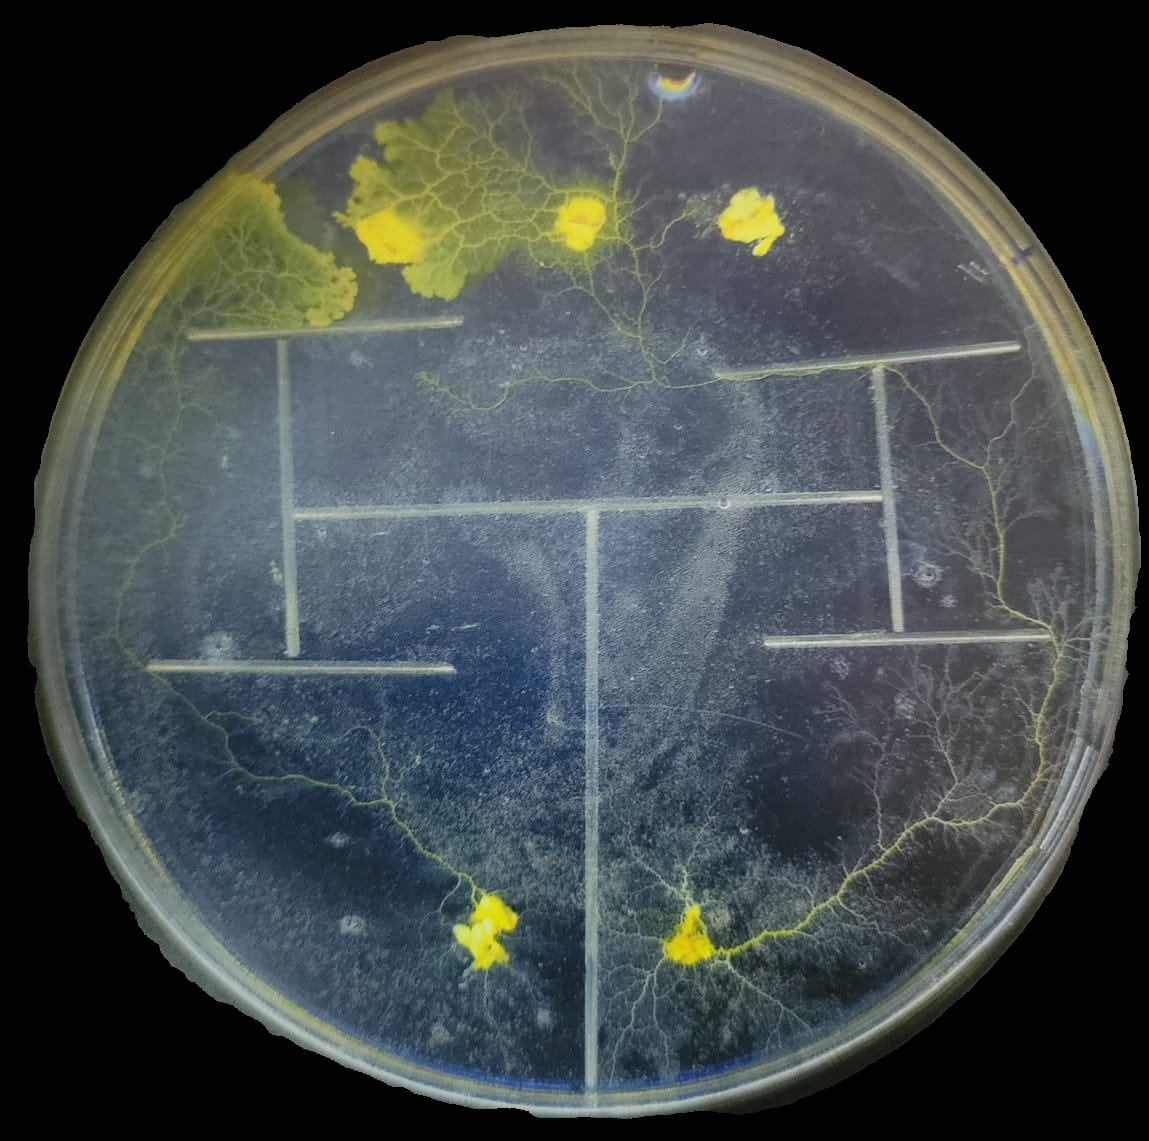
\includegraphics[width=0.17\textwidth]{./images/marco_teorico/Physarum/LaberintoPhysarum.png}
        \caption{Physarum Polycephalum resolviendo un laberinto. \cite{Adamatzky2014}.}
        \label{fig:PhysarumPolycephalum02}
    \end{wrapfigure}
    \vskip 0.5cm
    %Parrafo 3
    El Physarum Polycephalum es un organismo que se encuentra en la naturaleza en lugares h\'umedos y oscuros, 
        como en el interior de los troncos de los \'arboles en descomposici\'on, en hojarasca h\'umeda, en suelos 
        ricos en materia org\'anica y en lugares oscuros y h\'umedos. Este organismo se alimenta de bacterias, 
        hongos y otros microorganismos que se encuentran en su entorno, y se desplaza por medio de la contracci\'on 
        de sus fibras de actina, que le permiten moverse en busca de alimento.\cite{Dee1960}
    \vskip 0.5cm
    %Parrafo 4
    El Physarum Polycephalum es un organismo muy interesante para el estudio de la biolog\'ia y la f\'isica, 
        ya que tiene propiedades \'unicas que lo hacen un organismo muy especial. Por ejemplo, el Physarum Polycephalum 
        es capaz de resolver laberintos como se observa en la figura \ref{fig:PhysarumPolycephalum02}, encontrar la ruta m\'as corta entre dos puntos, y tomar decisiones complejas 
        basadas en la informaci\'on que recibe de su entorno. Adem\'as, el Physarum Polycephalum es capaz de aprender 
        y recordar informaci\'on, y de adaptarse a su entorno de una manera muy eficiente.
    \vskip 0.5cm
    %Parrafo 5
    Una vez dada una breve introducci\'on al Physarum Polycephalum, podemos pasar a la perspectiva de la computaci\'on, 
        en donde el Physarum Polycephalum ha sido utilizado para resolver problemas de optimizaci\'on, simulaci\'on 
        de redes de transporte, y modelado de sistemas complejos. En la siguiente secci\'on veremos c\'omo el Physarum 
        Polycephalum ha sido utilizado en la computaci\'on y en la modelaci\'on de sistemas complejos.
    